\section{Approche génétique}

\subsection{Que sont les algorithmes génétiques ?}

Les algorithmes génétiques sont des méthodes évolutionnistes qui simulent une évolution naturelle, génération après génération, où les individus peuvent muter, se croiser ou se reproduire (cloner).

Ils permettent, lorsqu'il n'existe pas de méthode exacte (ou que la solution est inconnue), d'obtenir une solution approchée en un temps raisonnable.

Dans ce projet, nous nous basons sur une librairie Python qui s'appelle \textit{Deap}.

\subsection{Instanciation de la classe et lancement de la méthode}

\begin{lstlisting}
s = GeneticScheduler(machines_list, jobs_list)
\end{lstlisting}

Le constructeur de la classe prend comme arguments la liste des machines et la liste des jobs que renvoie le parseur.

\begin{lstlisting}
s.run_genetic(total_population=10, max_generation=100, verbose=True)
\end{lstlisting}

Pour lancer l'algorithme, la métode \textit{run\_genetic} prend comme paramètres le nombre total d'individus dans la population, la génération maximale et si l'utilisateur souhaite activer la sortie standard ou non. Tous ces paramètres sont facultatifs et valent respectivement $10$, $100$ et \textit{True} par défaut.

\subsection{Création d'un individu}

\lstinputlisting[firstline=35, lastline=37]{./app/geneticscheduler.py}

Afin de trouver un individu initial, nous réalisons une copie profonde de la liste des jobs et des machines. En effet, ces dernières seront modifiées par le \textit{scheduler} de la partie précédente ce qui empêcherait toute autre simulation par la suite. 

\lstinputlisting[firstline=39, lastline=41]{./app/geneticscheduler.py}

Le \textit{scheduler} est ensuite appelé sur les listes temporaires précédemment créer en utilisant une heuristique de choix aléatoire pour les opérations afin d'augmenter la diversité de la population et éviter de converger vers un optimum local.

\lstinputlisting[firstline=43, lastline=49]{./app/geneticscheduler.py}

Comme l'opération a été réalisée sur des listes temporaires, il est nécessaire de faire la correspondance des activités et des opérations sur les listes initiales, les objets étant différents. Les couples \textit{activity} et \textit{operation} sont ensuite stockées dans une liste avec le temps auquel l'opération commence afin de pouvoir trier cette liste pour respecter la contrainte d'ordre.

\lstinputlisting[firstline=50, lastline=54]{./app/geneticscheduler.py}

La liste est donc triée par rapport au temps, puis on supprime cette composante de la liste pour créer notre individu. Les variables temporaires sont détruites et l'individu retourné.

\subsection{Création de la population initiale}

\lstinputlisting[firstline=56, lastline=58]{./app/geneticscheduler.py}

Notre population initiale correspond à $total\_population$ éléments. Chaque élement correspond à un individu retourné par la méthode \textit{init\_individual}.

\subsection{Evaluation de la fonction objectif d'un individu}

\lstinputlisting[firstline=107, lastline=108]{./app/geneticscheduler.py}

L'évaluation d'un individu est très simple. Comme nous souhaitons minimiser le temps total que mettent les jobs, l'évaluation correspond logiquement au temps que met l'individu pour terminer. Cette évaluation fait donc appel à la méthode \textit{compute\_time}. 

Cette évaluation repose sur une astuce. Comme les activités sont classées par ordre chronologique, il suffit de regarder à quel instant $t_1$ termine l'activité précédente du job et à quel instant $t_2$ termine la dernière activité sur la machine concernée par l'opération couramment considérée. Il suffit ensuite de prendre le max entre $t_1$ et $t_2$ pour avoir l'instant $t$ auquel l'activité commence.

\newpage

\lstinputlisting[firstline=61, lastline=71]{./app/geneticscheduler.py}

On initialise une liste contenant pour chaque activité le temps auquel elles commencent (utile pour la simulation finale) et deux dictionnaires, un premier faisant la correspondance entre $machine\_id$ et liste des opérations réalisées par cette mmachine, le deuxième faisant la même chose mais par rapport aux identifiants des jobs.

\lstinputlisting[firstline=73, lastline=94]{./app/geneticscheduler.py}

On calcule ensuite les instants de temps comme indiqué précédemment.

\newpage

\lstinputlisting[firstline=96, lastline=104]{./app/geneticscheduler.py}

Pour calculer le temps total que prend le planning, on regarde pour chaque machine le moment où la dernière opération commence ainsi que sa durée et on prend la somme maximale. Enfin, on renvoie la durée totale et la liste des instants temporels.

\subsection{Mutation d'un individu}

\lstinputlisting[firstline=113, lastline=115]{./app/geneticscheduler.py}

Pour réaliser la mutation d'un individu, on regarde les activités qui peuvent muter, autrement dit celles où plusieurs opérations sont possibles pour les réaliser.

\lstinputlisting[firstline=117, lastline=124]{./app/geneticscheduler.py}

S'il existe de telles activités, on en choisit une au hasard, et pour cette activité on choisit une opération différente. 

\lstinputlisting[firstline=125, lastline=128]{./app/geneticscheduler.py}

On supprime la composante \textit{fitness} (qui correspond à la fonction objective) car sa valeur n'est plus à jour et on renvoie le mutant.

\subsection{Permutation sur un individu}

Une permutation sur un individu correspond à une permutation de deux couples activité/opération ne violant pas la contrainte d'ordre. 

Exemple de planning en identifiant les activités par \textit{(id\_job, id\_activity)}:

\begin{figure}[!h]
    \centering
    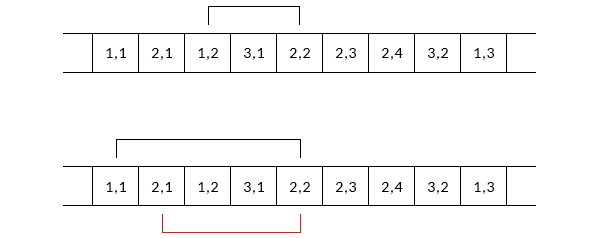
\includegraphics[scale=0.8]{report/Pictures/permutation.png}
\end{figure}

Par exemple, la première permutation est valide car elle respecte la contrainte d'ordre. Cependant, pour la deuxième, la contrainte d'ordre ne serait plus respectée car si j'échange le $(1,1)$ et le $(2,2)$, alors on aurait $(2,2)$ avant $(2,1)$ ce qui est impossible, de même avec $(1,1)$ et $(1,2)$. 

\lstinputlisting[firstline=135, lastline=147]{./app/geneticscheduler.py}

\newpage

Cette méthode permet de calculer les bornes min et max de permutation pour une activité donnée, autrement dit l'intervalle où l'on peut déplacer une activité sans que cela viole la contrainte d'ordre.

\lstinputlisting[firstline=149, lastline=170]{./app/geneticscheduler.py}

Tant que l'on a pas trouvé une permutation possible, on sélectionne deux activités au hasard et on vérifie si elles sont permutables, c'est à dire si chacune appartient au domaine de permutation de l'autre. Une fois cette permutation trouvée, elle est effectuée et le nouvel individu est renvoyé.

Il est à noter qu'une permutation est forcément possible à partir du moment où le nombre de jobs est au moins égal à deux.

\newpage

\subsection{Déplacement d'une activité au sein d'un individu}

\lstinputlisting[firstline=173, lastline=185]{./app/geneticscheduler.py}

Plutôt que de permuter deux activités, il est également possible de choisir une activité, de calculer ses bornes de déplacements valides et de la déplacer dans cette intervalle. Cette opération diffère de la permutation dans le sens où l'ordre des autres éléments n'est pas modifié.

\subsection{Évolution d'un individu}

\lstinputlisting[firstline=187, lastline=195]{./app/geneticscheduler.py}

Un individu donné peut muté, subir une permutation, ou les deux. On calcule pour cela deux probabilités, une par opération possible. Bien que par construction ces opérations respectent forcément la contrainte d'ordre, on effectue une vérification sur le futur individu.

\subsection{Simulation sur les machines d'un individu}

\lstinputlisting[firstline=190, lastline=198]{./app/geneticscheduler.py}

Pour un individu donné, on simule son exécution afin de pouvoir le dessiner éventuellement.

\subsection{Déroulement de l'algorithme}

\lstinputlisting[firstline=201, lastline=212]{./app/geneticscheduler.py}

Lors de l'appel de la méthode \textit{run\_genetic}, on commence par désactiver la sortie standard si demandé puis on initialise la libraire \textit{Deap}. On indique que l'on chercher à minimiser la fonction objectif. On enregistre également auprès de \textit{Deap} nos fonctions de création, de mutation, de permutation et d'évolution.

\lstinputlisting[firstline=214, lastline=215]{./app/geneticscheduler.py}

On crée ensuite notre population initiale.

\lstinputlisting[firstline=217, lastline=237]{./app/geneticscheduler.py}

On simule l'évolution pour $max\_generation$ générations. On définit les probabilités de mutations et de permutation puis on fait évoluer notre population et enfin on évalue la fonction objectif de chaque individu. Si un individu a une fonction objectif plus faible que \textit{best}, alors cet individu devient le meilleur individu. De plus, pour augmenter l'efficacité de notre algorithme vers la convergence de l'optimum, nous avons décidé de remplacer la population actuelle par une population composée uniquement du meilleur individu.

\newpage

\lstinputlisting[firstline=239, lastline=251]{./app/geneticscheduler.py}

On affiche les résultats et on simule le meilleur planning trouvé. On réactive la sortie standard si besoin.